\chapter{Appendix} \label{appendix}

\section{Limit Infeasible Curtail Action Experiment Results}

\begin{figure}[H]
	\centering
	\subfloat{}{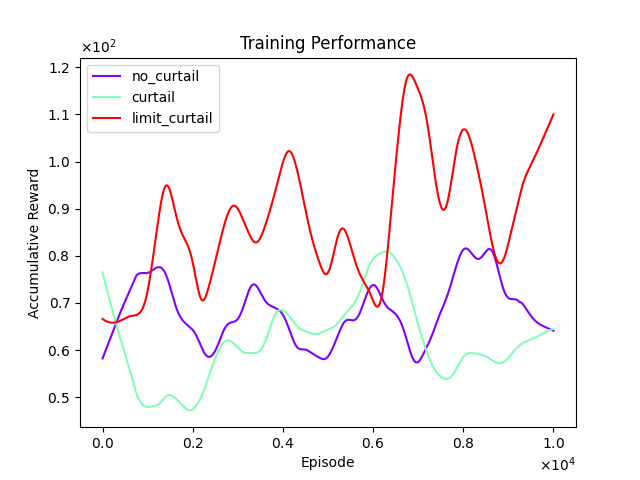
\includegraphics[width=.45\textwidth]{graphs/curtail_limit/training_performance.png}}
	\hskip1ex
	\subfloat{}{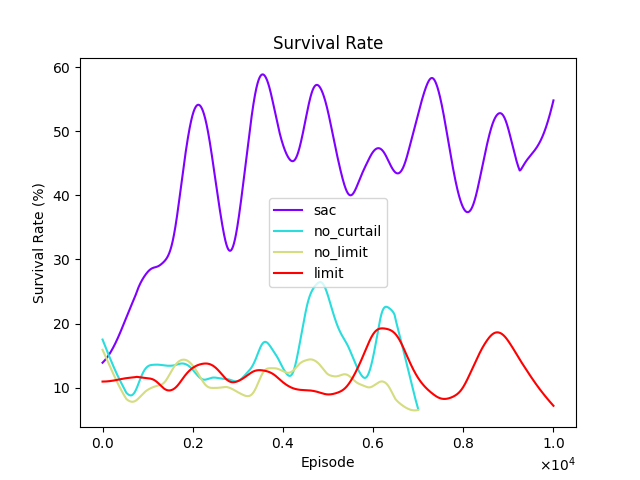
\includegraphics[width=.45\textwidth]{graphs/curtail_limit/survival_rate.png}} 
	\vfill
	\subfloat{}{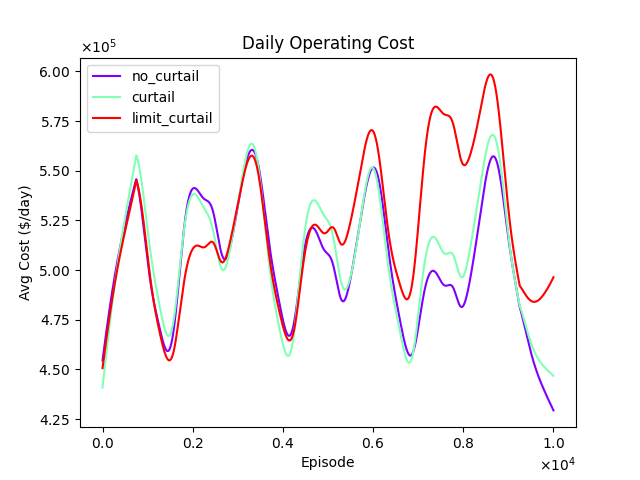
\includegraphics[width=.45\textwidth]{graphs/curtail_limit/daily_cost.png}} \hskip1ex
	\subfloat{}{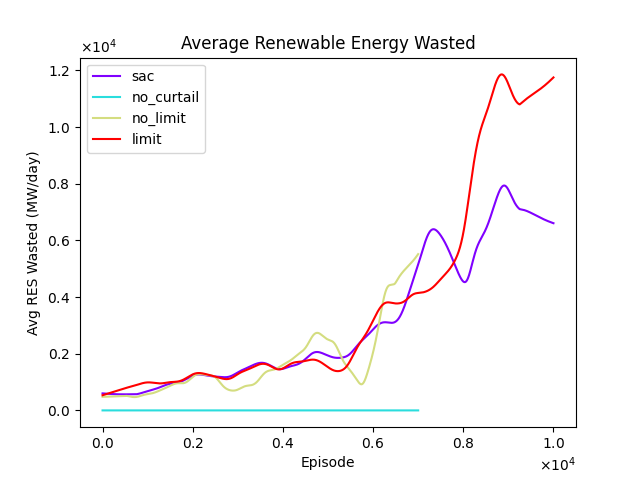
\includegraphics[width=.45\textwidth]{graphs/curtail_limit/res_wasted.png}} 
	\caption{Training Results of the Experiments concerning Limit Infeasible Curtail Actions.}
	\label{fig:curtail-train}
\end{figure}

\begin{table}[ht]
	\centering
	\begin{tabularx}{\textwidth}{|l|X|X|X|X|X|}
		\hline
		\textbf{Model} & \textbf{Avg. Accumulative Reward}& \textbf{Avg. Length (Steps)} & \textbf{Avg Daily Operating Cost (€)} & \textbf{Avg. Renewables Wasted (MW/day)} & \textbf{Total Time (Seconds)}\\
		\hline
		no\_curtail & 68.87 & 225.46 & 533238.32 & 0.0 & 812.81\\
		curtail & 60.81 & 108.27 & 551028.29 & 4565.01 & 510.97 \\
		limit\_curtail & 78.62 & 759.82 & 575798.57 & 7640.76 & 2329.76 \\
		\hline
	\end{tabularx}
	\caption{Validation Results of the Experiments concerning Limit Infeasible Curtail Actions.}
	\label{fig:curtail-val}
\end{table}

\section{Curtailment Lower Limit Smoothing}

\begin{figure}[H]
	\centering
	\subfloat{}{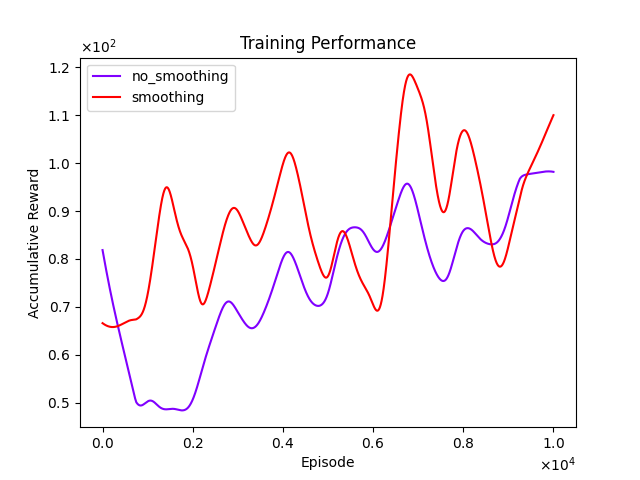
\includegraphics[width=.45\textwidth]{graphs/curtail_smooth/training_performance.png}}
	\hskip1ex
	\subfloat{}{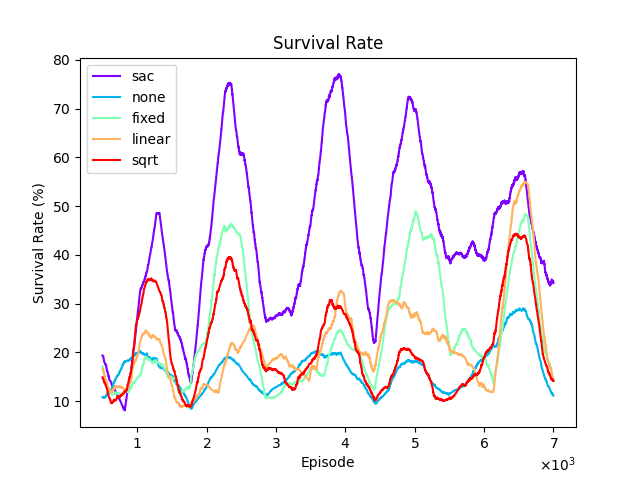
\includegraphics[width=.45\textwidth]{graphs/curtail_smooth/survival_rate.png}} 
	\vfill
	\subfloat{}{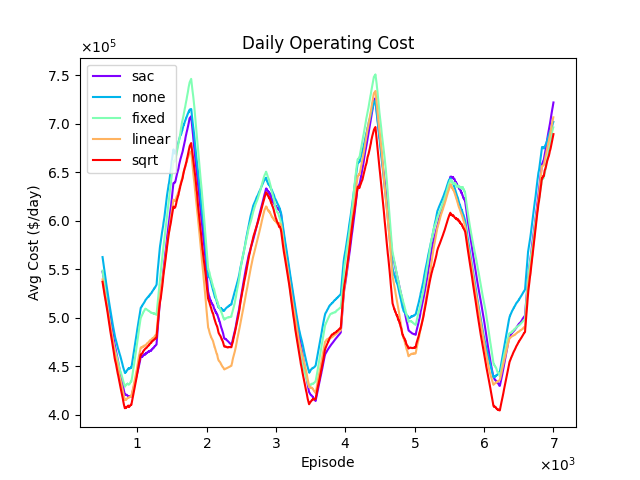
\includegraphics[width=.45\textwidth]{graphs/curtail_smooth/daily_cost.png}} \hskip1ex
	\subfloat{}{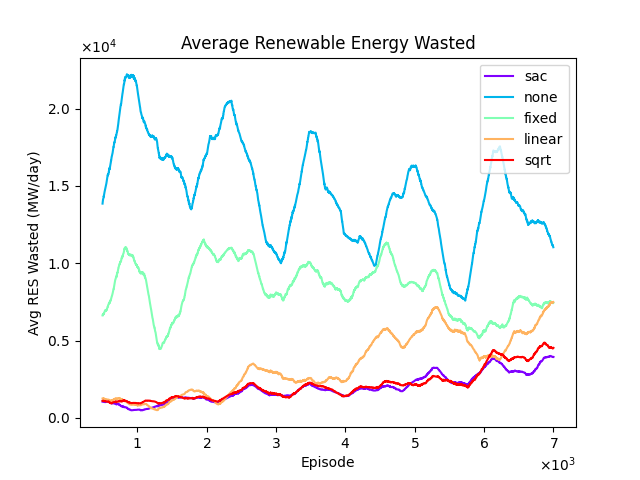
\includegraphics[width=.45\textwidth]{graphs/curtail_smooth/res_wasted.png}} 
	\caption{Training Results of the Experiments concerning Curtailment Lower Limit Smoothing.}
	\label{fig:curtail-smooth-train}
\end{figure}

\begin{table}[ht]
	\centering
	\begin{tabularx}{\textwidth}{|l|X|X|X|X|X|}
		\hline
		\textbf{Model} & \textbf{Avg. Accumulative Reward}& \textbf{Avg. Length (Steps)} & \textbf{Avg Daily Operating Cost (€)} & \textbf{Avg. Renewables Wasted (MW/day)} & \textbf{Total Time (Seconds)}\\
		\hline
		no\_smoothing & 94.91 & 476.48 & 565094.39 & 10106.84 & 3011.93 \\
		smoothing & 78.62 & 759.82 & 575798.57 & 7640.76 & 2329.76 \\
		\hline
	\end{tabularx}
	\caption{Validation Results of the Experiments concerning Limit Infeasible Curtail Actions.}
	\label{fig:curtail-val}
\end{table}

\section{Reward Experiments}

\begin{figure}[H]
	\centering
	\subfloat{}{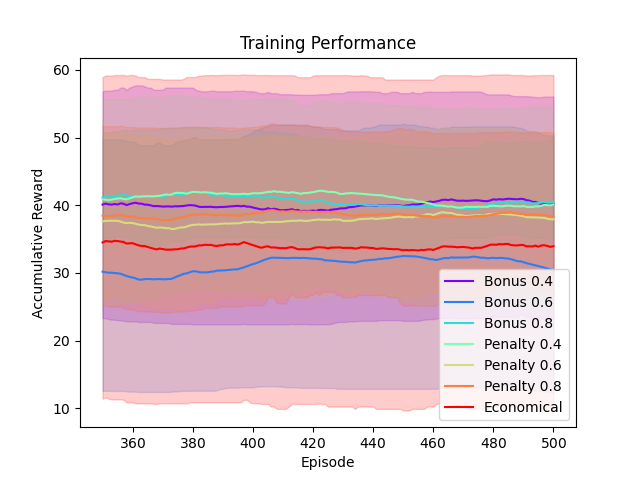
\includegraphics[width=.45\textwidth]{graphs/reward/training_performance.png}}
	\hskip1ex
	\subfloat{}{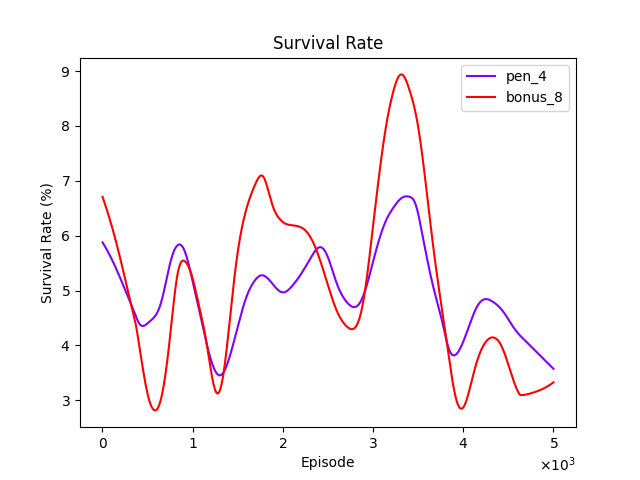
\includegraphics[width=.45\textwidth]{graphs/reward/survival_rate.png}} 
	\vfill
	\subfloat{}{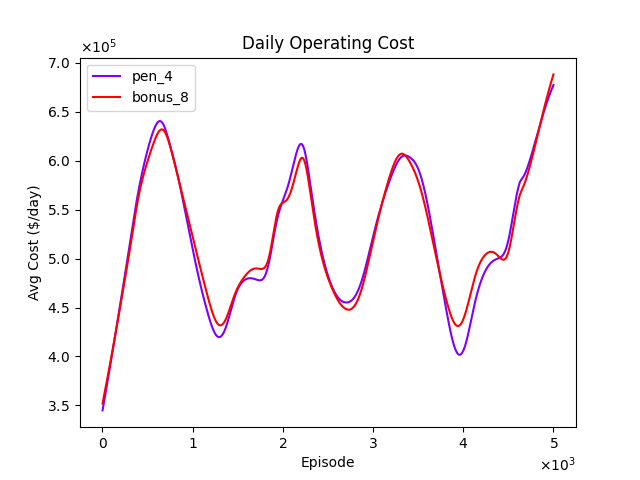
\includegraphics[width=.45\textwidth]{graphs/reward/daily_cost.png}} \hskip1ex
	\subfloat{}{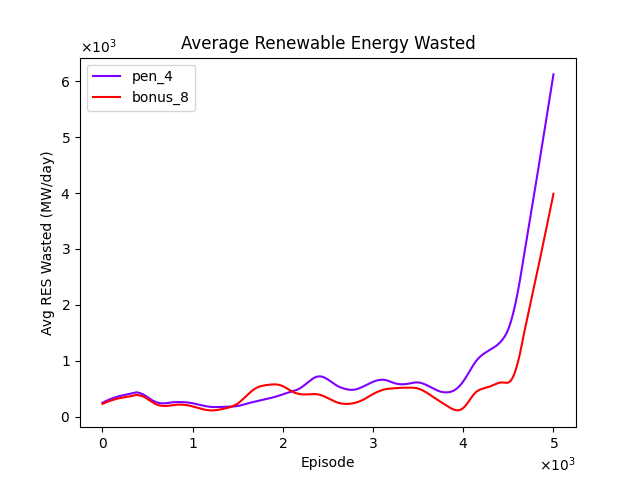
\includegraphics[width=.45\textwidth]{graphs/reward/res_wasted.png}} 
	\caption{Training Results of the best Penalty and Bonus Factor Rewards.}
	\label{fig:reward-best-train}
\end{figure}
\begin{figure}[H]
	\centering
	\subfloat{}{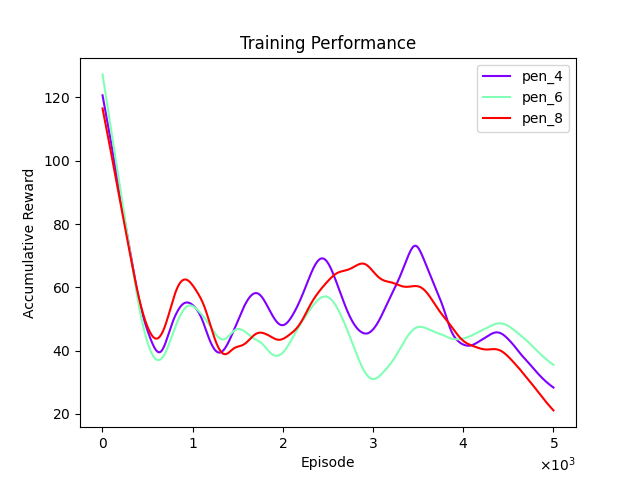
\includegraphics[width=.45\textwidth]{graphs/reward/penalty/training_performance.png}}
	\hskip1ex
	\subfloat{}{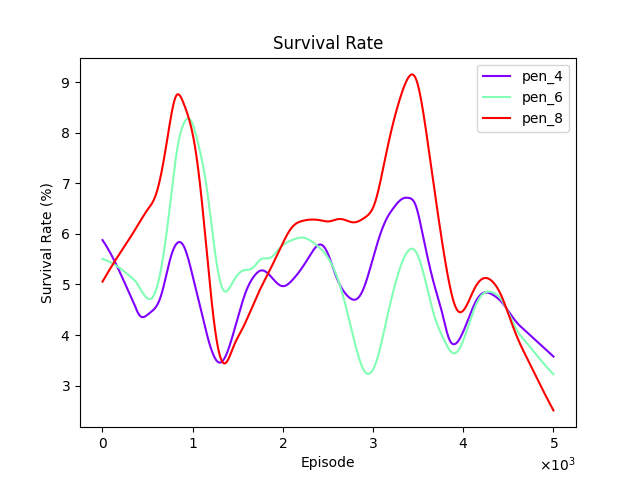
\includegraphics[width=.45\textwidth]{graphs/reward/penalty/survival_rate.png}} 
	\vfill
	\subfloat{}{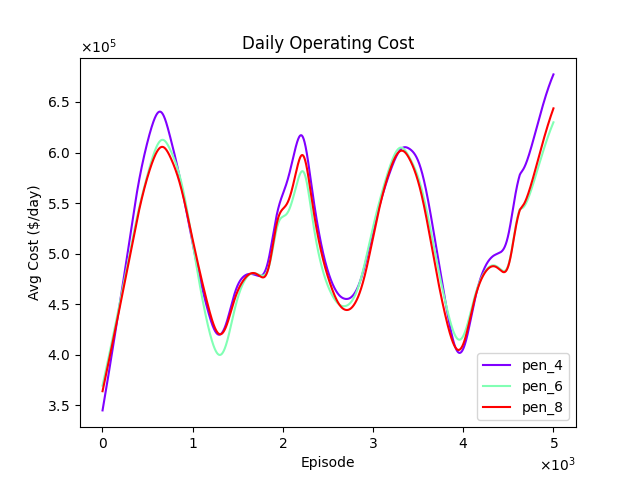
\includegraphics[width=.45\textwidth]{graphs/reward/penalty/daily_cost.png}} \hskip1ex
	\subfloat{}{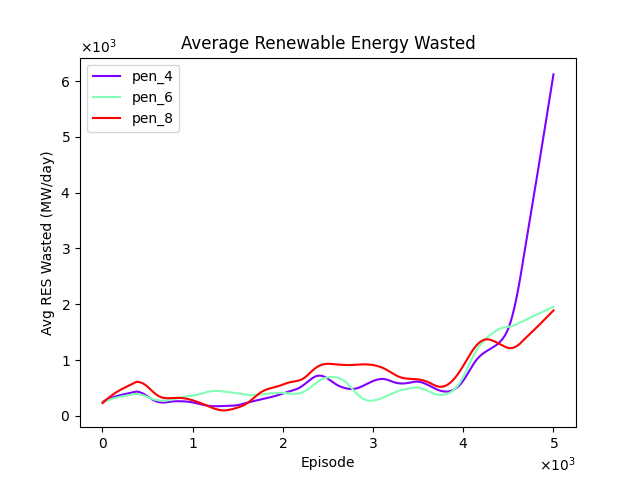
\includegraphics[width=.45\textwidth]{graphs/reward/penalty/res_wasted.png}} 
	\caption{Training Results of the Penalty Factor Rewards.}
	\label{fig:reward-pen-train}
\end{figure}

\begin{figure}[H]
	\centering
	\subfloat{}{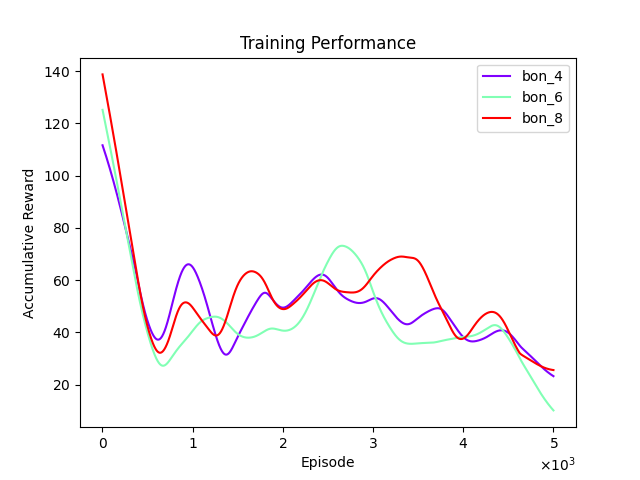
\includegraphics[width=.45\textwidth]{graphs/reward/bonus/training_performance.png}}
	\hskip1ex
	\subfloat{}{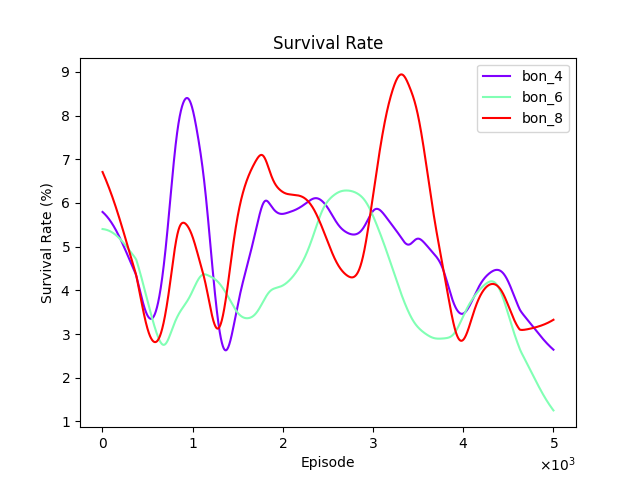
\includegraphics[width=.45\textwidth]{graphs/reward/bonus/survival_rate.png}} 
	\vfill
	\subfloat{}{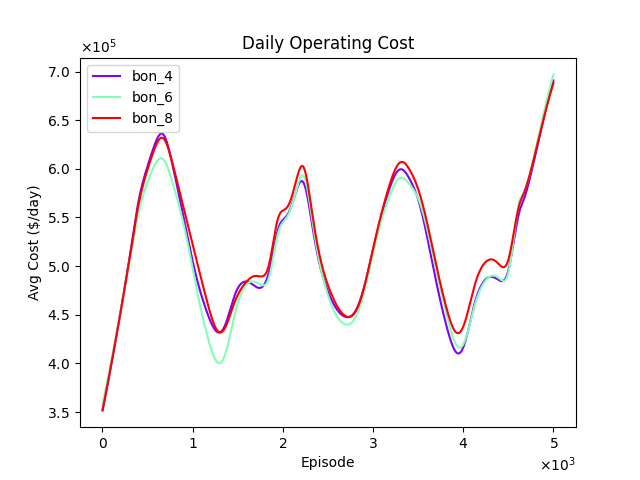
\includegraphics[width=.45\textwidth]{graphs/reward/bonus/daily_cost.png}} \hskip1ex
	\subfloat{}{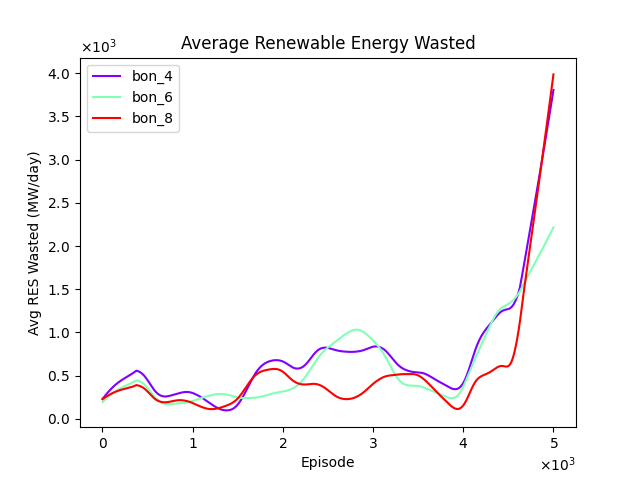
\includegraphics[width=.45\textwidth]{graphs/reward/bonus/res_wasted.png}} 
	\caption{Training Results of the Bonus Factor Rewards.}
	\label{fig:reward-bon-train}
\end{figure}

\begin{table}[ht]
	\centering
	\begin{tabularx}{\textwidth}{|l|X|X|X|X|X|}
		\hline
		\textbf{Model} & \textbf{Avg. Accumulative Reward}& \textbf{Avg. Length (Steps)} & \textbf{Avg Daily Operating Cost (€)} & \textbf{Avg. Renewables Wasted (MW/day)} & \textbf{Total Time (Seconds)}\\
		\hline
		pen\_4 & 40.57 & 80.75 & 565893.63 & 4100.20 & 230.99 \\
		pen\_6 & 37.54 & 81.40 & 558362.82 & 2570.71 & 231.09 \\
		pen\_8 & 38.22 & 76.35 & 555582.14 & 2612.34 & 222.58 \\
		bon\_4 & 40.13 & 76.23 & 565757.16 & 3723.72 & 223.90 \\
		bon\_6 & 30.78 & 55.06 & 566786.07 & 2750.34 & 189.01 \\
		bon\_8 & 40.88 & 96.43 & 560927.60 & 3115.18 & 256.59 \\
		\hline
	\end{tabularx}
	\caption{Validation Results of the Experiments concerning Limit Infeasible Curtail Actions.}
	\label{fig:curtail-val}
\end{table}

\section{Experiments on the \ac{GNN} Tuning}

\begin{table}
	\begin{tabular}{|l|l|}
		\hline
		\textbf{Parameter} & \textbf{Values} \\
		\hline
		Aggregation Function & \{'sum','mean', 'min', 'max', 'mul'\} \\
		\hline
		Number of Layers & \{1,2,3,4,5\} \\
		\hline
		Hidden Channels & \{6, 12, 18, 24, 36\} \\
		\hline
		Ouput Channels & \{3, 6, 12, 18, 24, 36\} \\
		\hline 
		Dropout Rate & [0.1, 0.4] \\
		\hline
		Activation First & {True, False} \\
		\hline 
		Heads & {1,2,3,6} \\
		\hline
		GATv2 & {True, False} \\
		\hline
	\end{tabular}
	\caption{General \ac{GNN} Parameters Tuned}
\end{table}

\begin{table}
	\begin{tabular}{|l|l|l|}
		\hline
		\textbf{Implementation} & \textbf{Parameter} & \textbf{Values} \\
		\hline
		GCN & Improved & {True, False} \\
		\hline 
		GAT & Heads & {1,2,3,6} \\
		\hline
		GAT & GATv2 & {True, False} \\
		\hline
	\end{tabular}
	\caption{Model-Specific Parameters Tuned}
\end{table}

\section{Experiments on the \ac{GNN} Parameters \textit{act\_first} and \textit{improved}}

\begin{figure}[H]
	\centering
	\subfloat{}{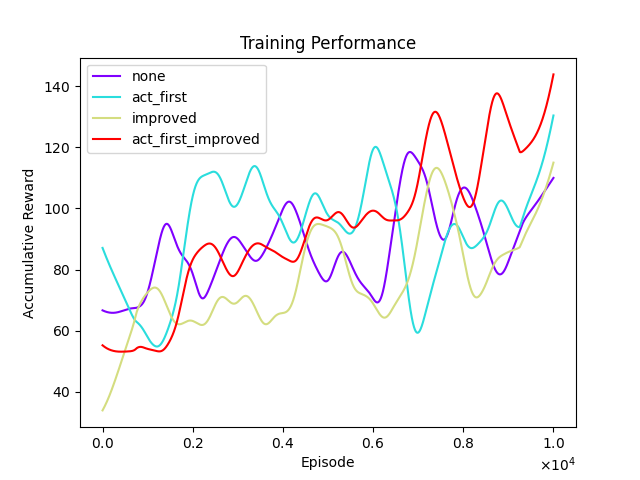
\includegraphics[width=.45\textwidth]{graphs/act_first_improved/training_performance.png}}
	\hskip1ex
	\subfloat{}{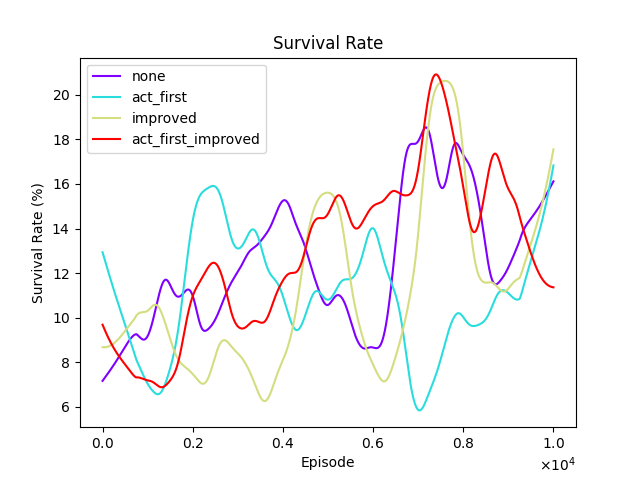
\includegraphics[width=.45\textwidth]{graphs/act_first_improved/survival_rate.png}} 
	\vfill
	\subfloat{}{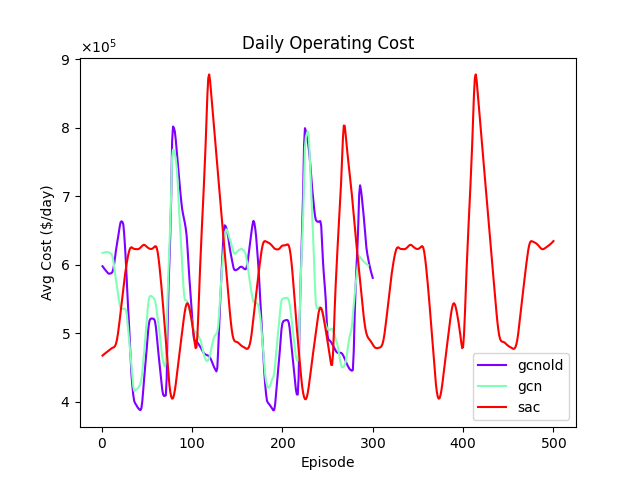
\includegraphics[width=.45\textwidth]{graphs/act_first_improved/daily_cost.png}} \hskip1ex
	\subfloat{}{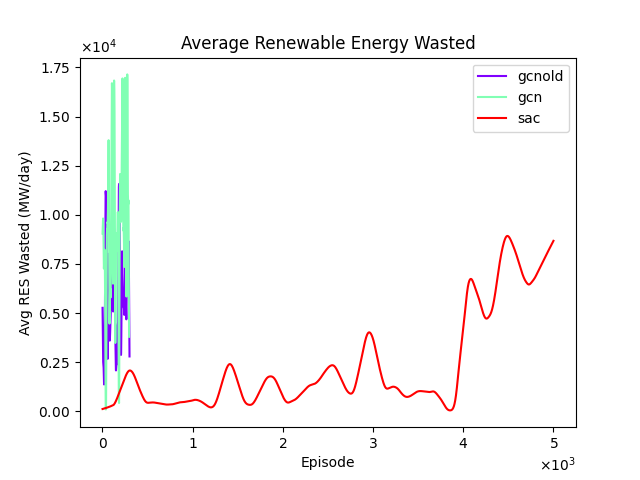
\includegraphics[width=.45\textwidth]{graphs/act_first_improved/res_wasted.png}} 
	\caption{Training Results of the act\_first and improved Parameter Tests.}
	\label{fig:act-first-improved-train}
\end{figure}

\begin{comment}
\begin{table}[ht]
	\centering
	\begin{tabularx}{\textwidth}{|l|X|X|X|X|X|}
		\hline
		\textbf{Model} & \textbf{Avg. Accumulative Reward}& \textbf{Avg. Length (Steps)} & \textbf{Avg Daily Operating Cost (€)} & \textbf{Avg. Renewables Wasted (MW/day)} & \textbf{Total Time (Seconds)}\\
		\hline
		none & & & & & \\
		act\_first & & & & & \\
		improved & & & & & \\
		act\_first\_improved & & & & &  \\
		\hline
	\end{tabularx}
	\caption{Validation Results of the Experiments concerning Limit Infeasible Curtail Actions.}
	\label{fig:curtail-val}
\end{table}
\end{comment}

\section{Experiments on the \ac{GCN} Aggregation Function} \label{appendix:aggr}

\begin{table}
	\begin{tabular}{|l|l|}
		\hline
		\textbf{Parameter} & \textbf{Values} \\
		\hline
		Aggregation Function & \{'sum','mean', 'min', 'max', 'mul'\} \\
		\hline
		Number of Layers & 1 \\
		\hline
		Hidden Channels & 18 \\
		\hline
		Ouput Channels & 6 \\
		\hline 
		Dropout Rate & 0.1 \\
		\hline
		Activation First & True \\
		\hline
	\end{tabular}
	\caption{Parameters of Aggregation Function Experiment}
	\label{table:aggr-params}
\end{table}

\begin{figure}[H]
	\centering
	\subfloat{}{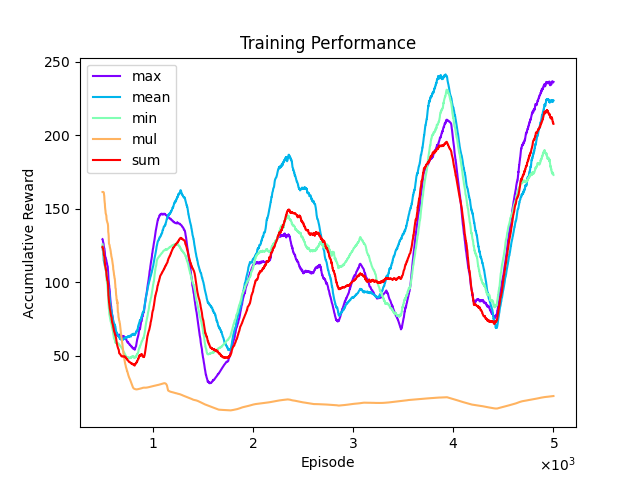
\includegraphics[width=.45\textwidth]{graphs/aggr/training_performance.png}}
	\hskip1ex
	\subfloat{}{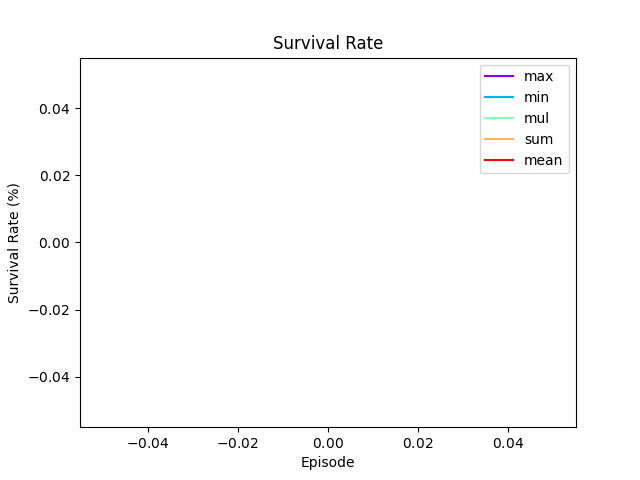
\includegraphics[width=.45\textwidth]{graphs/aggr/survival_rate.png}} 
	\vfill
	\subfloat{}{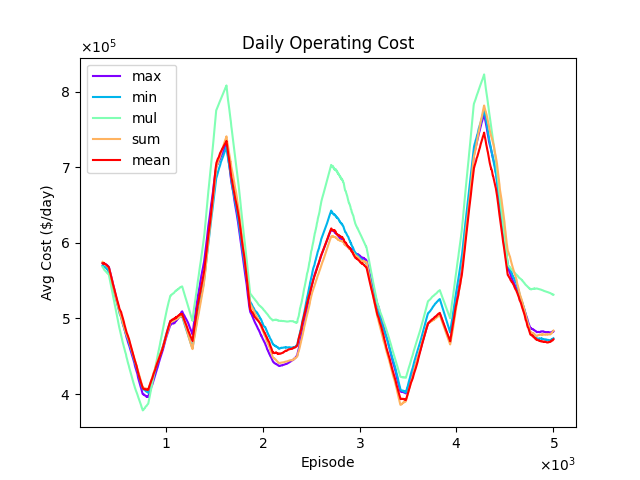
\includegraphics[width=.45\textwidth]{graphs/aggr/daily_cost.png}} \hskip1ex
	\subfloat{}{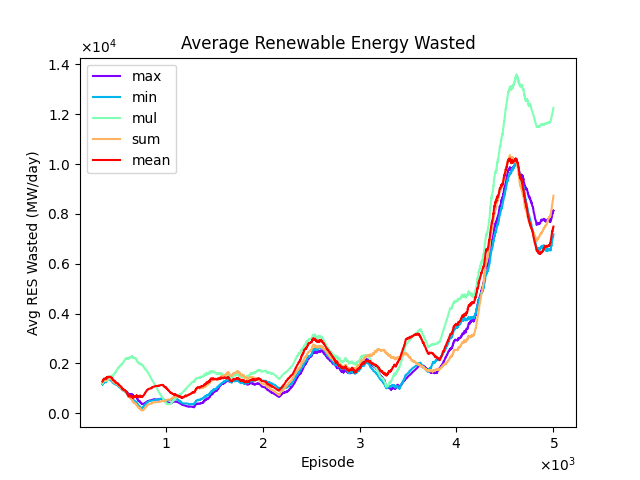
\includegraphics[width=.45\textwidth]{graphs/aggr/res_wasted.png}} 
	\caption{Training Results of different types of \ac{GNN} aggregation functions}
	\label{fig:aggr-train}
\end{figure}

	\begin{table}[ht]
		\centering
		\begin{tabularx}{\textwidth}{|l|X|X|X|X|X|}
			\hline
			\textbf{Model} & \textbf{Avg. Accumulative Reward}& \textbf{Avg. Length (Steps)} & \textbf{Avg Daily Operating Cost (€)} & \textbf{Avg. Renewables Wasted (MW/day)} & \textbf{Total Time (Seconds)}\\
			\hline
			max & 119.16 & 677.75 & 560219.45 & 6564.49 & 552.51\\
			sum & 114.58 & 768.58 & 569952.37 & 7268.28 &  606.28 \\
			mean & 92.90 &  551.24 & 557637.84 & 6268.06 & 454.24 \\
			min & 80.89 & 495.70 & 559033.63 & 6687.94 & 416.63 \\
			mul & 15.76 & 1104.06 & 608319.66 & 10305.96 & 846.43 \\
			\hline
		\end{tabularx}
		\caption{Validation Results of different types of \ac{GNN} aggregation functions.}
		\label{table:aggr-val}
	\end{table}

\section{Experiments on the number of \ac{GCN} layers}

\begin{table}
	\begin{tabular}{|l|l|}
		\hline
		\textbf{Parameter} & \textbf{Values} \\
		\hline
		Aggregation Function & 'max' \\
		\hline
		Number of Layers & [1, 6] \\
		\hline
		Hidden Channels & 18 \\
		\hline
		Ouput Channels & 6 \\
		\hline 
		Dropout Rate & 0.1 \\
		\hline
		Activation First & True \\
		\hline 
		\hline
	\end{tabular}
	\caption{General \ac{GNN} Parameters Tuned}
\end{table}

\begin{figure}[H]
	\centering
	\subfloat{}{\includegraphics[width=.45\textwidth]{graphs/layers/training_performance.png}}
	\hskip1ex
	\subfloat{}{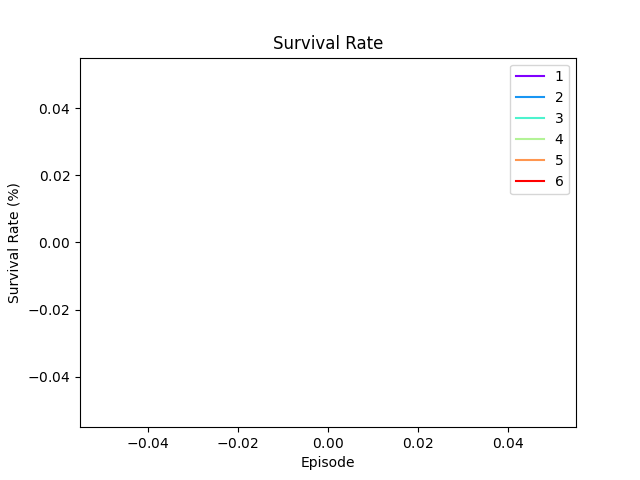
\includegraphics[width=.45\textwidth]{graphs/layers/survival_rate.png}} 
	\vfill
	\subfloat{}{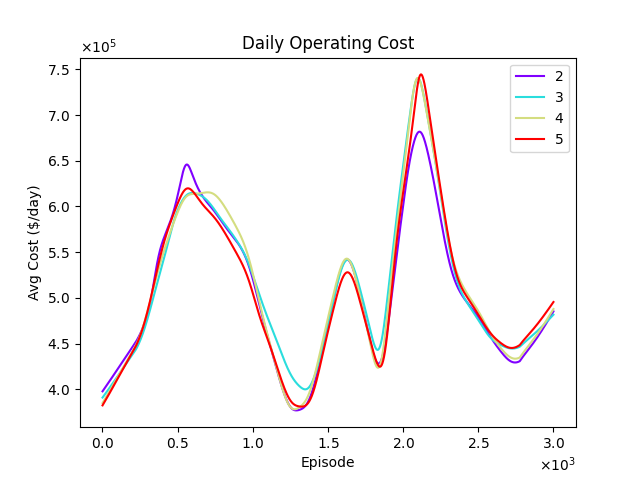
\includegraphics[width=.45\textwidth]{graphs/layers/daily_cost.png}} \hskip1ex
	\subfloat{}{\includegraphics[width=.45\textwidth]{graphs/layers/res_wasted.png}} 
	\caption{Training Results of models with 2, 3, 4 and 5 \ac{GNN} Layers}
	\label{fig:gnn-layers-train}
\end{figure}


\begin{table}[ht]
	\centering
	\begin{tabularx}{\textwidth}{|l|X|X|X|X|X|}
		\hline
		\textbf{Model} & \textbf{Avg. Accumulative Reward}& \textbf{Avg. Length (Steps)} & \textbf{Avg Daily Operating Cost (€)} & \textbf{Avg. Renewables Wasted (MW/day)} & \textbf{Total Time (Seconds)}\\
		\hline
		6 & 135.75 & 487.09 & 560147.77 & 5862.49 & 655.44 \\
		3 & 110.73 & 736.32 & 567510.58 & 7116.24 & 744.50 \\
		1 & 101.24 & 709.76 & 565865.82 & 6855.58 & 573.30 \\
		4 & 98.67 & 451.51 & 577464.90 & 8641.05 & 529.76 \\
		5 & 92.97 & 286.65 & 550205.21 & 6397.41 & 386.19 \\
		2 & 91.58 & 694.67 & 575093.64 & 5989.95 & 638.11 \\
		\hline
	\end{tabularx}
	\caption{Validation Results of the Experiments concerning Limit Infeasible Curtail Actions.}
	\label{fig:curtail-val}
\end{table}


\section{Experiments on the number of \ac{GAT} Heads}

\begin{figure}[H]
	\centering
	\subfloat{}{\includegraphics[width=.45\textwidth]{graphs/layers/training_performance.png}}
	\hskip1ex
	\subfloat{}{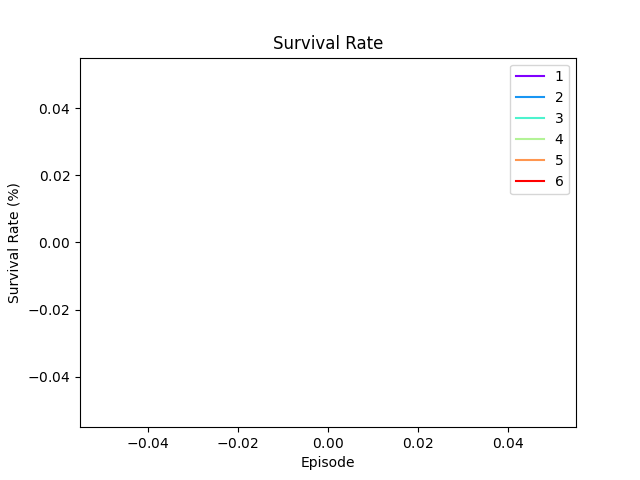
\includegraphics[width=.45\textwidth]{graphs/layers/survival_rate.png}} 
	\vfill
	\subfloat{}{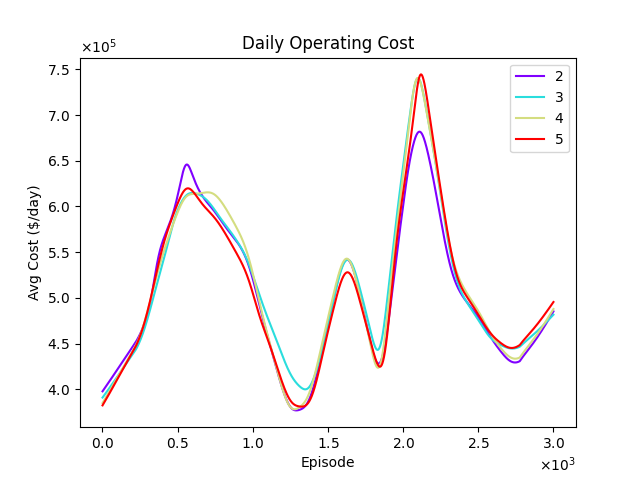
\includegraphics[width=.45\textwidth]{graphs/layers/daily_cost.png}} \hskip1ex
	\subfloat{}{\includegraphics[width=.45\textwidth]{graphs/layers/res_wasted.png}} 
	\caption{Training Results of models with 1, 2 and 3 \ac{GAT} Heads}
	\label{fig:gat-heads-train}
\end{figure}

\begin{comment}
\begin{table}[ht]
	\centering
	\begin{tabularx}{\textwidth}{|l|X|X|X|X|X|}
		\hline
		\textbf{Model} & \textbf{Avg. Accumulative Reward}& \textbf{Avg. Length (Steps)} & \textbf{Avg Daily Operating Cost (€)} & \textbf{Avg. Renewables Wasted (MW/day)} & \textbf{Total Time (Seconds)}\\
		\hline
		1 & & & & & \\
		2 & & & & & \\
		3 & & & & & \\
		\hline
	\end{tabularx}
	\caption{Validation Results of the Experiments concerning Limit Infeasible Curtail Actions.}
	\label{fig:curtail-val}
\end{table}
\end{comment}

\section{GNNs vs. SAC Experiments}

\begin{figure}[H]
	\centering
	\subfloat{}{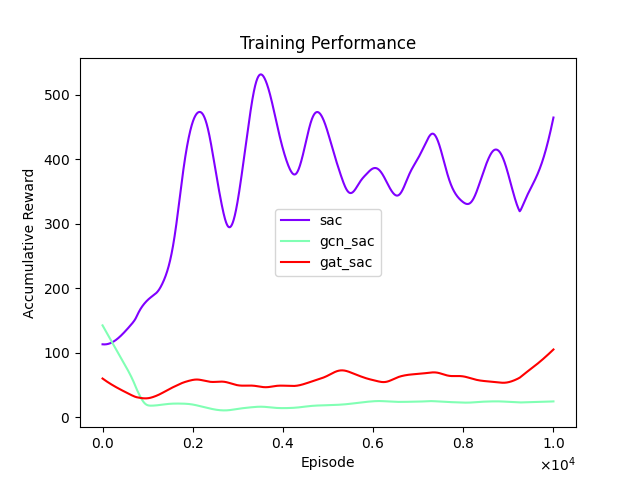
\includegraphics[width=.45\textwidth]{graphs/gnns/training_performance.png}}
	\hskip1ex
	\subfloat{}{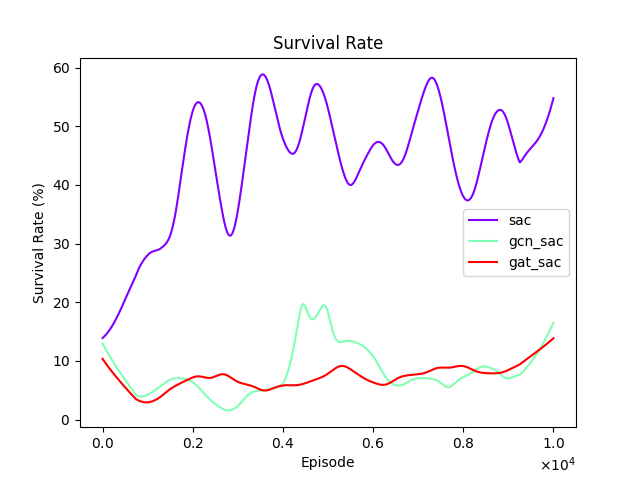
\includegraphics[width=.45\textwidth]{graphs/gnns/survival_rate.png}} 
	\vfill
	\subfloat{}{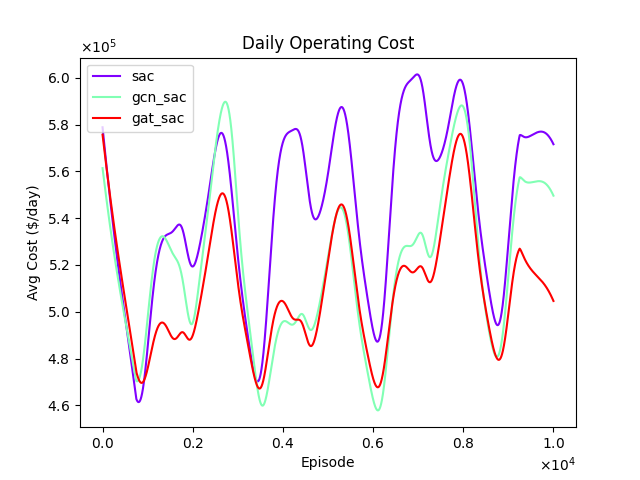
\includegraphics[width=.45\textwidth]{graphs/gnns/daily_cost.png}} \hskip1ex
	\subfloat{}{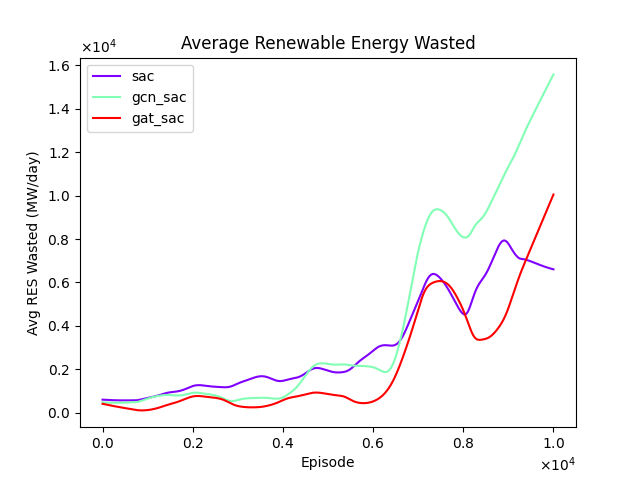
\includegraphics[width=.45\textwidth]{graphs/gnns/res_wasted.png}} 
	\caption{Training Results of models with 1, 2 and 3 \ac{GAT} Heads}
	\label{fig:gnns-train}
\end{figure}

	\begin{table}[ht]
		\centering
		\begin{tabularx}{\textwidth}{|l|X|X|X|X|X|}
			\hline
			\textbf{Model} & \textbf{Avg. Accumulative Reward}& \textbf{Avg. Length (Steps)} & \textbf{Avg Daily Operating Cost (€)} & \textbf{Avg. Renewables Wasted (MW/day)} & \textbf{Total Time (Seconds)}\\
			\hline
			sac & 342.84 & 1118.24 & 601896.44 & 5443.64 & 741.23 \\
			gcn\_sac & 23.38 & 573.73 & 549592.13 & 9885.84 & 467.29 \\
			gat\_sac & 55.80 & 481.72  & 553388.36 & 6064.43 & 603.91 \\
			\hline
		\end{tabularx}
		\caption{Validation Results of the Experiments concerning Limit Infeasible Curtail Actions.}
		\label{fig:curtail-val}
	\end{table}


\begin{comment}
\section{Experiments on 118-bus scenario}

\begin{figure}[H]
	\centering
	\subfloat{}{\includegraphics[width=.45\textwidth]{graphs/scale/training_performance.png}}
	\hskip1ex
	\subfloat{}{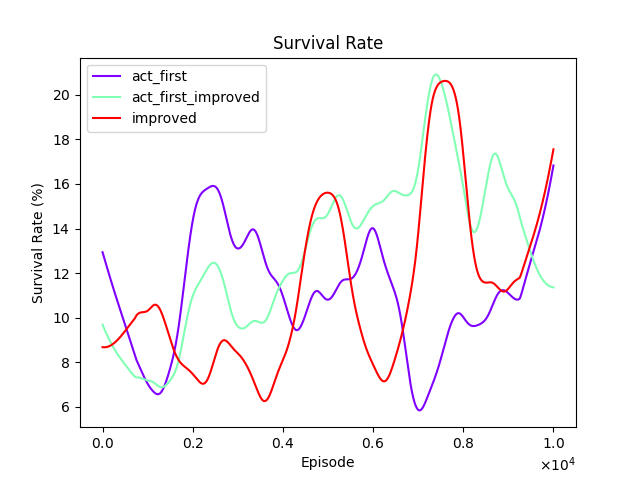
\includegraphics[width=.45\textwidth]{graphs/scale/survival_rate.png}} 
	\vfill
	\subfloat{}{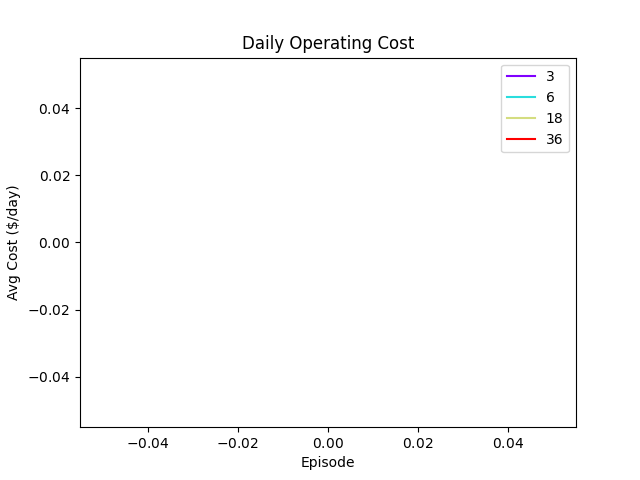
\includegraphics[width=.45\textwidth]{graphs/scale/daily_cost.png}} \hskip1ex
	\subfloat{}{\includegraphics[width=.45\textwidth]{graphs/scale/res_wasted.png}} 
	\caption{Training Results of models with 1, 2 and 3 \ac{GAT} Heads}
	\label{fig:118-train}
\end{figure}


	\begin{table}[ht]
		\centering
		\begin{tabularx}{\textwidth}{|l|X|X|X|X|X|}
			\hline
			\textbf{Model} & \textbf{Avg. Accumulative Reward}& \textbf{Avg. Length (Steps)} & \textbf{Avg Daily Operating Cost (€)} & \textbf{Avg. Renewables Wasted (MW/day)} & \textbf{Total Time (Seconds)}\\
			\hline
			sac & 81.98 & 361.917 & 2788763.38 & 4740.03 & 186.48 \\
			2
			gcn\_sac & 11.74 & 815.64 & 2679050.39 & 6567.22 & 318.94 \\
			\hline
		\end{tabularx}
		\caption{Validation Results of the Experiments concerning Limit Infeasible Curtail Actions.}
		\label{fig:curtail-val}
	\end{table}
	
	content...
	\end{comment}